
\chapter{Hand gesture Recognition System} \label{hgr}

\section{introduction}

in This chapters is organized as follows, First is the Preprocessing step we will build a system that can detect and track the Hand based on minimum depth detected by Kinect sensor,then filtering any minimum depth that is not the hand, after the preprocessing  a surf and sift descriptor are applied to get description of Gestures features  and fed them into an SVM kernel via a bag of features  Approach  (also called Bag of visual Words) to reduce dimensionality of surf and sift Features space by building a codebook for our gestures, another Approach was used which is Fourier shape Descriptor where we made a dictionary for feature extraction and then Classify gestures using Nearest neighbor classifier.

\section{Data Acquisition}

to build our HGR we must first acquire Gesture's images  using a sensor to represent data from the actual world space  to the numerical space, in our system we used Microsoft Kinect Sensor\ref{sec:kinect}  to acquire both RGB and depth images fpr the  16 different gestures performed by the signer, and building a datasets of 8000 images 500  for each gesture and divided later into three partitions as we will discuss later. 



\begin{figure}[H]
\centering
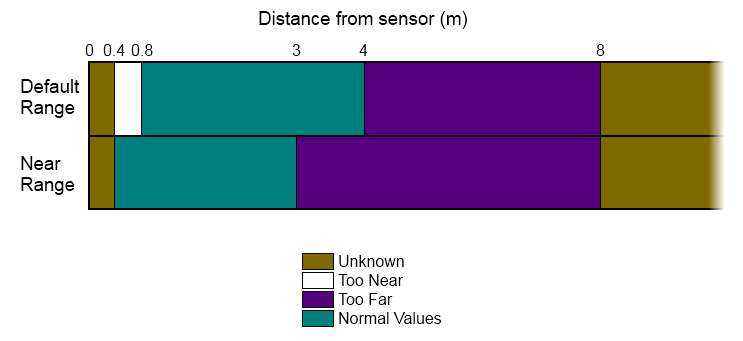
\includegraphics[width=0.8\textwidth]{img/dist.png}
\caption{Depth ranges}
\label{fig:dist}
\end{figure}



as we can see in \ref{fig:dist} the depth sensor  
can give distace data until 4 meters long, but For a better resolution  the user must be  in The \textbf{optimal distance } for our HGR system Which is practically between \textbf{[80 cm, 2,5m]} of course the closer the better but it is highly recommended  to not  be any lesser than 80 cm, However we chose maximal resolution 640 $\times$ 480 to have clear details of pixels,thereafter we make a crop to the image of size (271 $\times$ 211) because it gives us enough definition to distinguish the contour  of the hands.This choice greatly reduce the number of operations, and consequently, it will improve the efficiency of the code. 

\subsection{Depth space vs color Space }
A normal color camera can be used for sign language recognition but the problem comes when we want to use it for real time applications, in this case we have to track the hand position first and then we can go for recognition but implementing the hand tracking will involve complex algorithms which will make the overall system  computationally heavy, but with the kinect depth camera this task becomes easy as it has a skeleton tracking capability by using color and depth images so we can track the approximate hand position using the skeleton data, there are 20 joints that can be tracked these joints numbers are shown in \ref{table:t1}

\begin{table}[H]
\centering
\caption{JointType Enumeration}
 \label{table:t1} 
\begin{tabu} to 0.5\textwidth { | X[l] | X[r] | }

 \hline
 SpineMid = 1  & Neck = 2    \\
 \hline 
 Head = 3  &  ShoulderLeft = 4    \\
\hline
  ElbowLeft = 5   &  WristLeft = 6    \\
\hline

 HandLeft =	7  &   ShoulderRight = 8    \\
\hline
 
ElbowRight = 9  &  WristRight = 10   \\
\hline
 
 HandRight = 11  &  HipLeft = 12   \\
\hline
 
 KneeLeft = 13  &  AnkleLeft = 14   \\
\hline
 
FootLeft = 15  &  HipRight = 16   \\
\hline
 
 KneeRight = 17  & AnkleRight = 18     \\
\hline

FootRight = 19   & SpineShoulder = 20     \\

\hline

 \end{tabu}
 \end{table}

in the following figure \ref{fig:cam9} we will show the hand position both in color and depth space using Skeletal tracking  :

\begin{figure}[H]
\centering
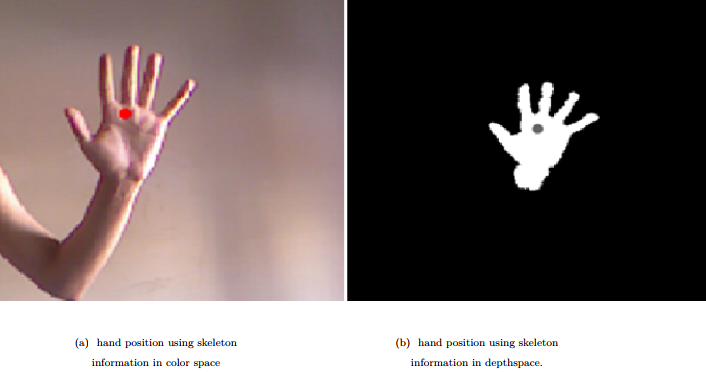
\includegraphics[width= 1.0\textwidth]{img/colorvsdepth.PNG}

\caption {Hand position's in both color image and depth image.
\label{fig:cam9}}
\end{figure}


By Using depth data   we eliminate all
sorts of confusion related to background. This also filters the cluttered background or overlapped images (i.e. hand overlapped with face) and illumination changes,  which justifies the use of depth sensor over RGB camera. In addition  the images of depth does not show enough contrast variations  in the hand region  so that we can get more discriminative keypoints to differentiate close gestures. 

\subsection{Vocabulary}
we performed 16 different gestures.

\begin{figure}[H]
\centering
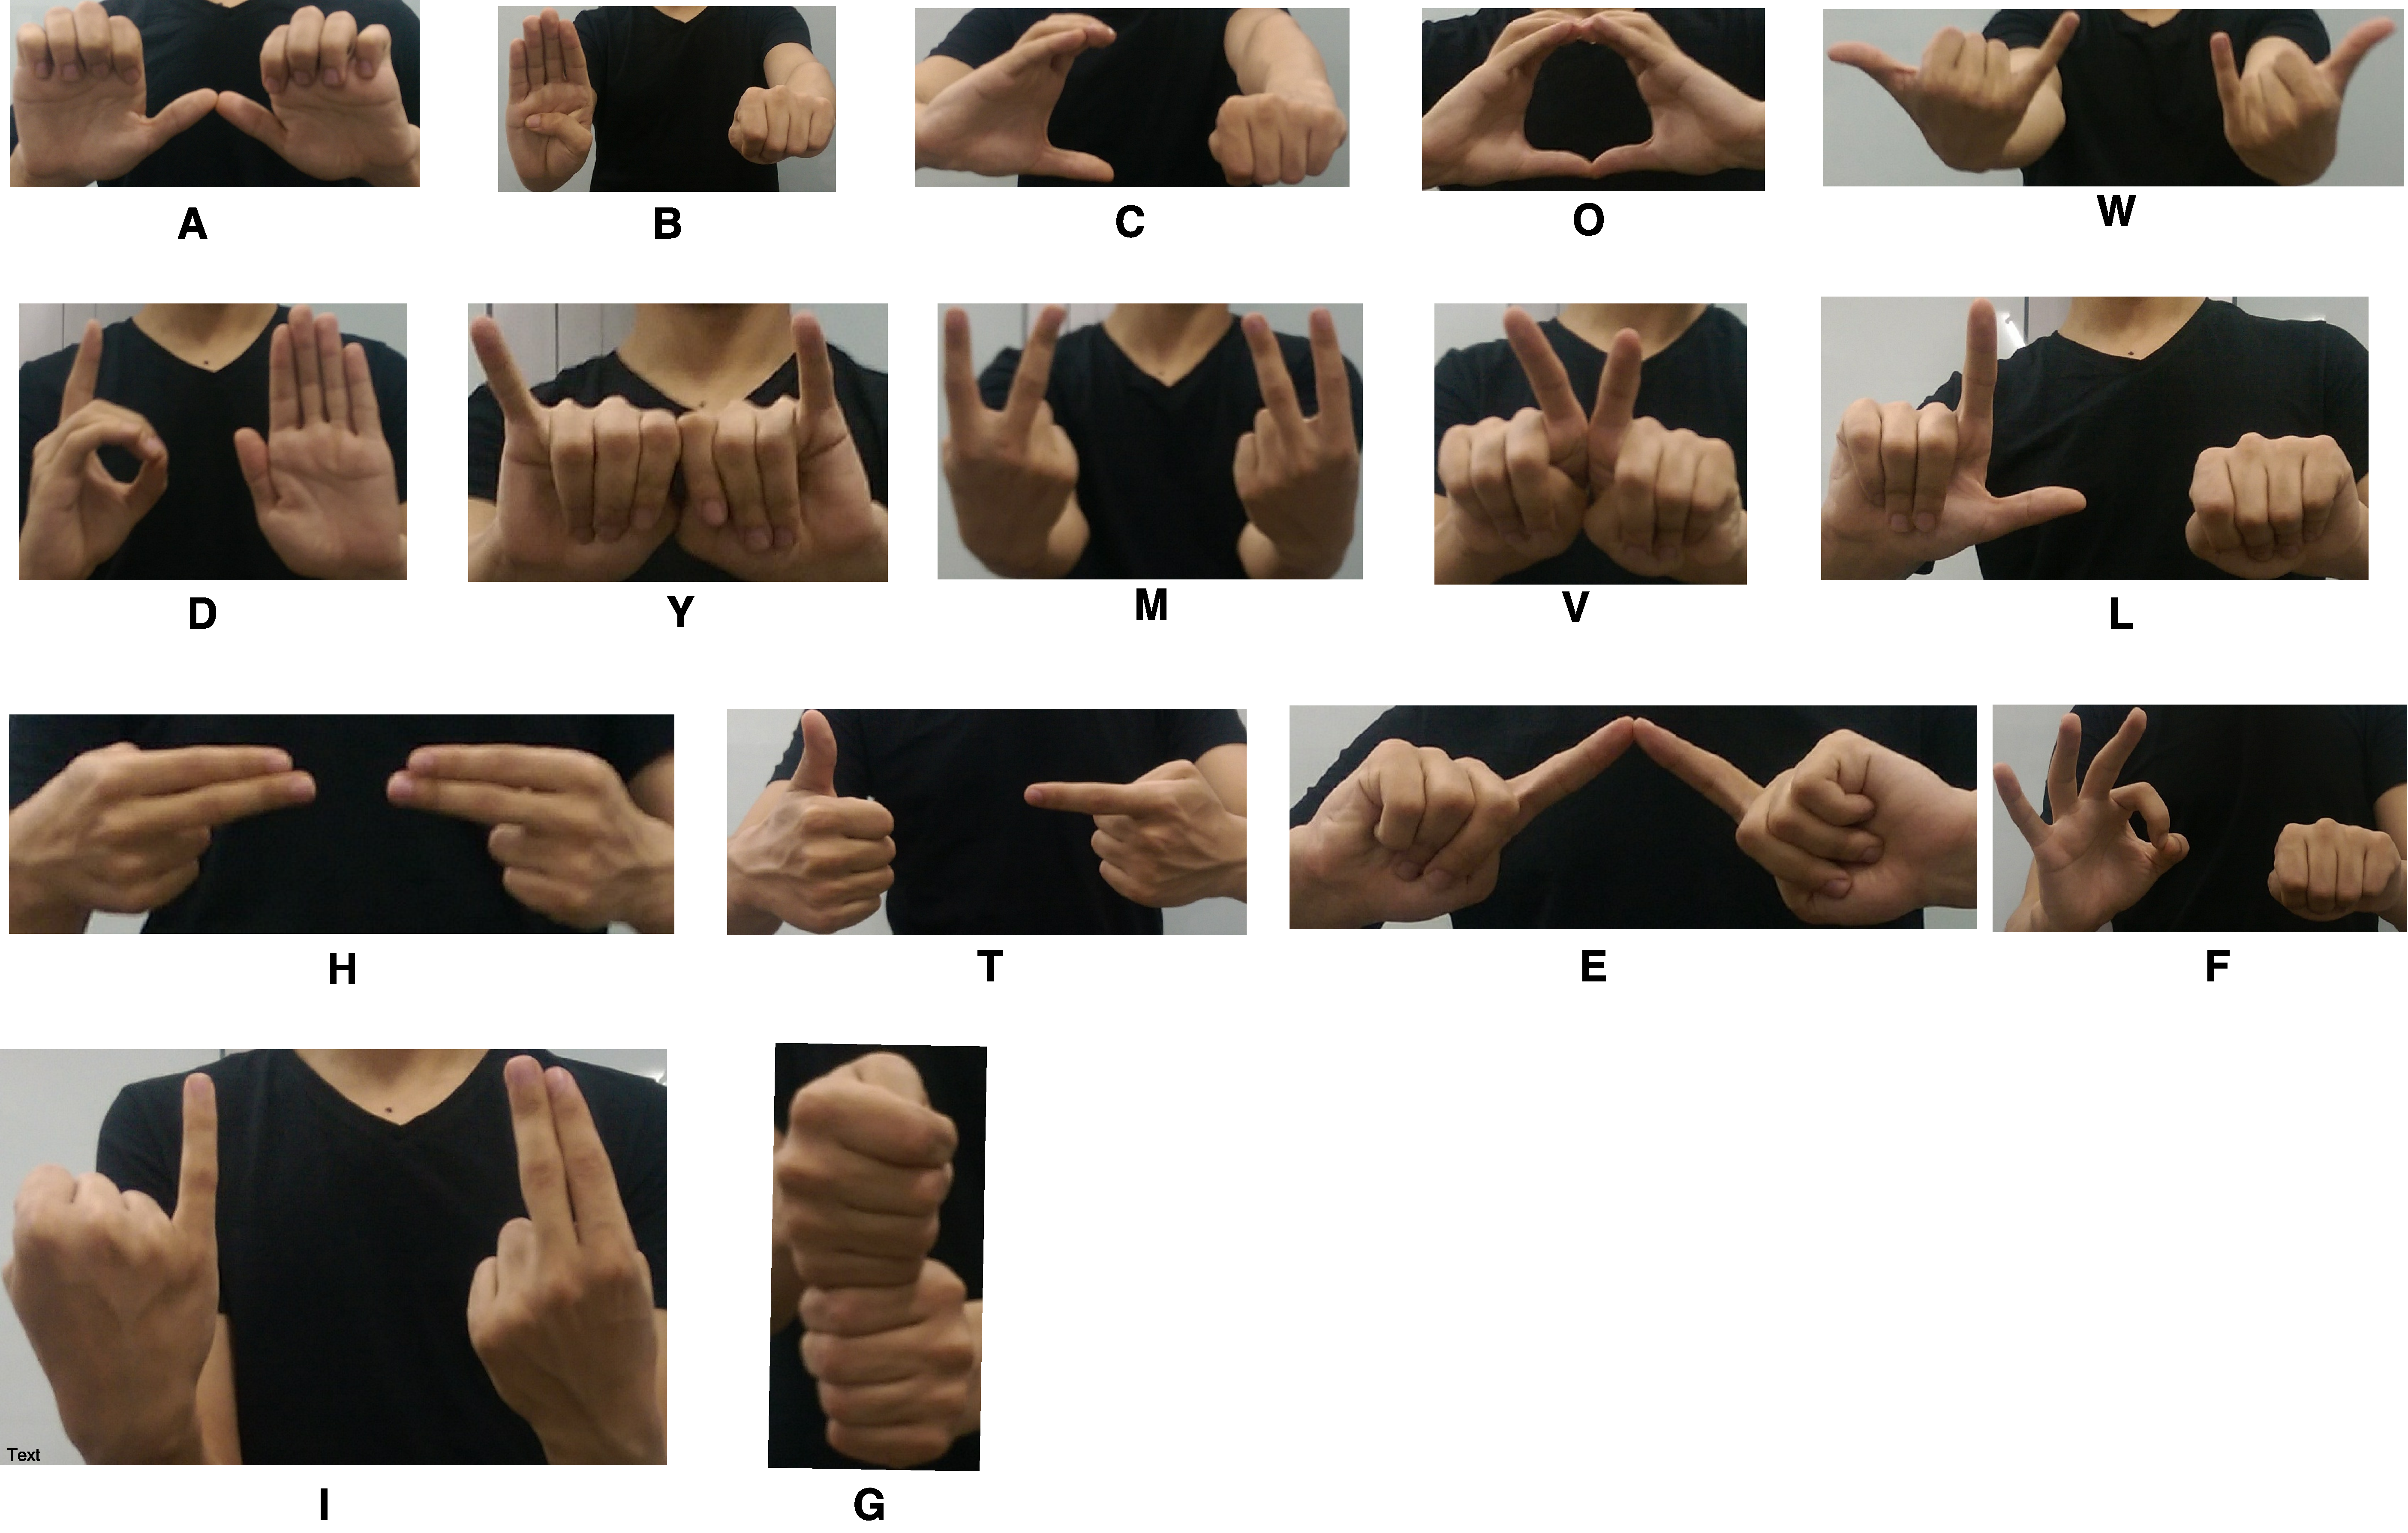
\includegraphics[width=1.0\textwidth]{img/vocab.pdf}
\caption{ Vocabulary dataset  }
\label{fig:vocab}
\end{figure}


\textcolor{blue}{ \textbf{Note :}} our Depth datasets is public for anyone to use  the link is at the bottom of the page.\footnote{\href{https://drive.google.com/file/d/0B89YnIYeclpadHF5ajVQVUJTTjg/view}{HGR-dataset}}



\section{Hand tracking And  detection}

\subsection{Relative depth }
The First step we need to accomplish in order to start to work with the depth data, is to decide which pixels are we going to take into account to carry on the tracking. The Kinect can catch the distance of the points which are visible to the camera, between the values \textbf{minDistance and maxDistance} (\ref{fig:cam8}).

\begin{figure}[H]
\centering
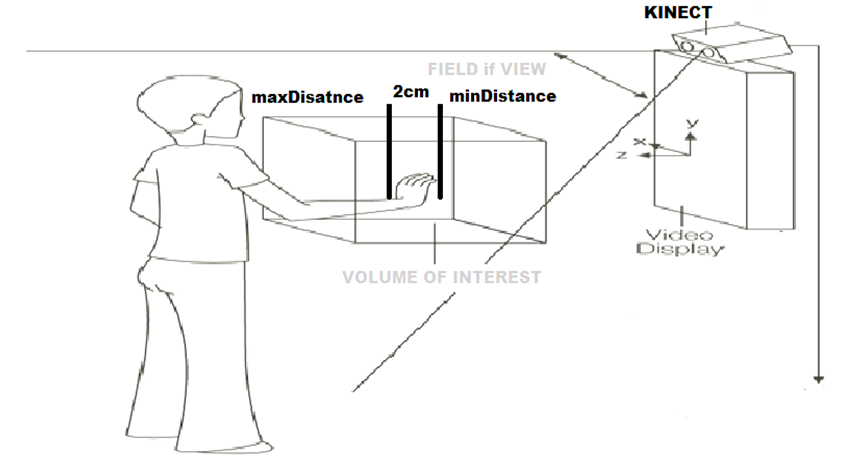
\includegraphics[width=1.0\textwidth]{img/mindistance.png}
\caption{Relative depth thresholding }
\label{fig:cam8}
\end{figure}

We are going to base our choice on the object’s proximity to the Kinect. We can choose if a pixel is near based on its depth  The lesser the depth the more likely it’s the hand region.\\\textbf{ Absolute depth}: A pixel is near if its depth is lesser than a constant value, that means that the pixel is between \textbf{minDistance }and a predefined value which is greater than \textbf{minDistance }and lesser than \textbf{maxDistance}.\\\textbf{Relative depth }:First of all,  we calculate the minimum depth, and  base on that depth we select a maximum depth (by adding a constant value to the minimum depth). So, if the depth is between these two values, the pixel is near. This method allow us to have greater mobility, because it does not force us to stay in the same position the whole time. 

\textbf{In the figure \ref{fig:cam8}} the minimum depth is \textbf{minDistance} and we add a tolerance of\textbf{  t= 2cm }to it, so every point between \textbf{minDistance and minDistance + t }  will be accepted as near, that's because the hand is not flat and uniform so this tolerance will handle that problem for us.


\subsection{Hand isolation using object connectivity }

After depth thresholding we notice that there are regions that do not belong to the hand, such as what appears to be one of my  arms or some furniture or my body when my hand is closer to my body like shown in the figure  \ref{fig:cam10}. These objects just happen to be on the same depth layer as my arm and hand this means that the Distance between these objects and the Kinect lies  between the range : $$[minDistance,minDistance +2cm] \pm {Error\ committed\ by\ Kinect\ } $$.


\begin{figure}[H]
\centering
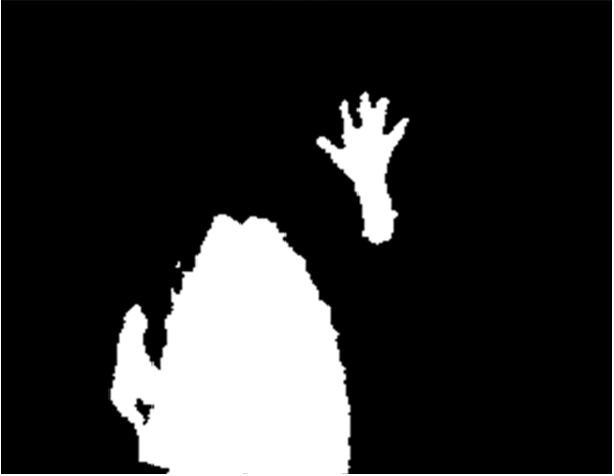
\includegraphics[width=0.5\textwidth]{img/depththresholding.png}
\caption{the depth of the body is in  the range [minDistance,minDistance +2cm]}
\label{fig:cam10}
\end{figure}

the approach used in this project  is to realize that most of the times, hands are not connected to any other object after the thresholding. We already know that the center region belongs to the hand from skeleton tracking, so we can simply apply`` floodfill ()`` offered by OpenCV to find all the connected image regions.

\textbf{ Definition and explanation of the algorithm used in floodfill () }

\begin{algorithm}[H]

\caption{Algorithm of Flood Fill }
\textbf{function}  Flood-fill(node,target\_color,replacement\_color)\\ 
\If{target\_color  ==  replacement\_color }
    {
     return
    }
\If{color of node \neq target\_color }
    {
     return
    }
Set the color of node to replacement$\_$color 

\textbf{Flood-fill}(one step to the west of node, target\_color, replacement\_color)\\
\textbf{Flood-fill}(one step to the east of node, target\_color, replacement\_color)\\
\textbf{Flood-fill}(one step to the north of node, target\_color, replacement\_color)\\
\textbf{Flood-fill}(one step to the south of node, target\_color, replacement\_color)\\
\textbf{return.} 
\end{algorithm}
with this simple algorithm we can separate objects from each other and therefor the following  Results : 
 
\begin{figure}[H]
\centering
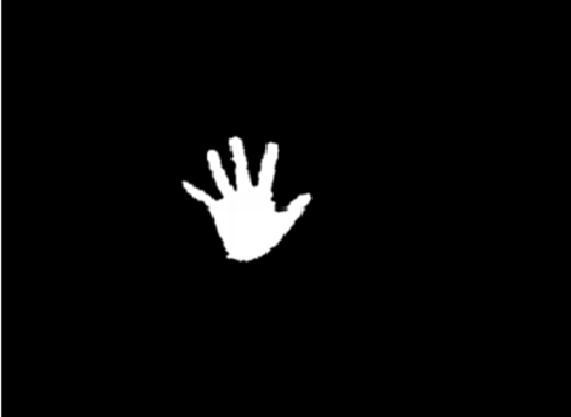
\includegraphics[width=0.5\textwidth]{img/finalresult.png}
\caption{result after applying connectivity check for one hand  }
\label{fig:cam11}
\end{figure}

the same process done with the other hand, Making an \textbf{OR } operation to the two images we end up having two hands isolated like shown in fig \ref{fig:twohd}

 \begin{figure}[H]
\centering
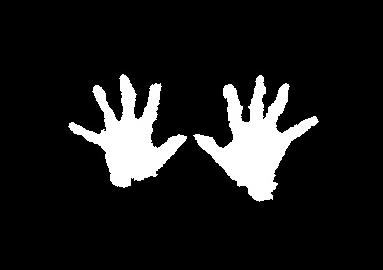
\includegraphics[width=0.5\textwidth]{img/twohands.jpg}
\caption{result after applying connectivity for both hands  }
\label{fig:twohd}
\end{figure}
now after finishing  the preprocessing phase, Since we are taking a resolution of 271 $\times$ 211 Pixels, to make sure the hands are being tracked we make a bounding box that is basically related to the left hand Position, this was made under the assumption that sign language  usually performed with two hands close to each other, \\
bounding box steps : 
\begin{itemize}
\item  Use LEFT hand location provided by SDK Skeleton  tracker (Px, Py)
 \item Crop to box around hand using depth at (Px, Py)
    \item scale = $\frac{20000.0f}{Depth(px,py)}$ 
    \begin{enumerate}
    \item Constant 20000.0f  found empirically
    \item Proportional to the area of bounding box 
    \end{enumerate}
\item Top left Pixel  = ( Px -10 * Scale * 0.5, Py - 10*Scale * 0.5)
\begin{enumerate}
    \item This formula scales an initial 10x10 box centered at (Px, Py) to
the appropriate dimensions based on the depth 
    \item Constants 0.5  take into account that most hand
silhouettes are more tall than wide 
    \end{enumerate}
   \item Width = Height = 10 * Scale 
\end{itemize}

\textcolor{blue}{\textbf{Summary of the section in below picture :} }

 \begin{figure}[H]
\centering
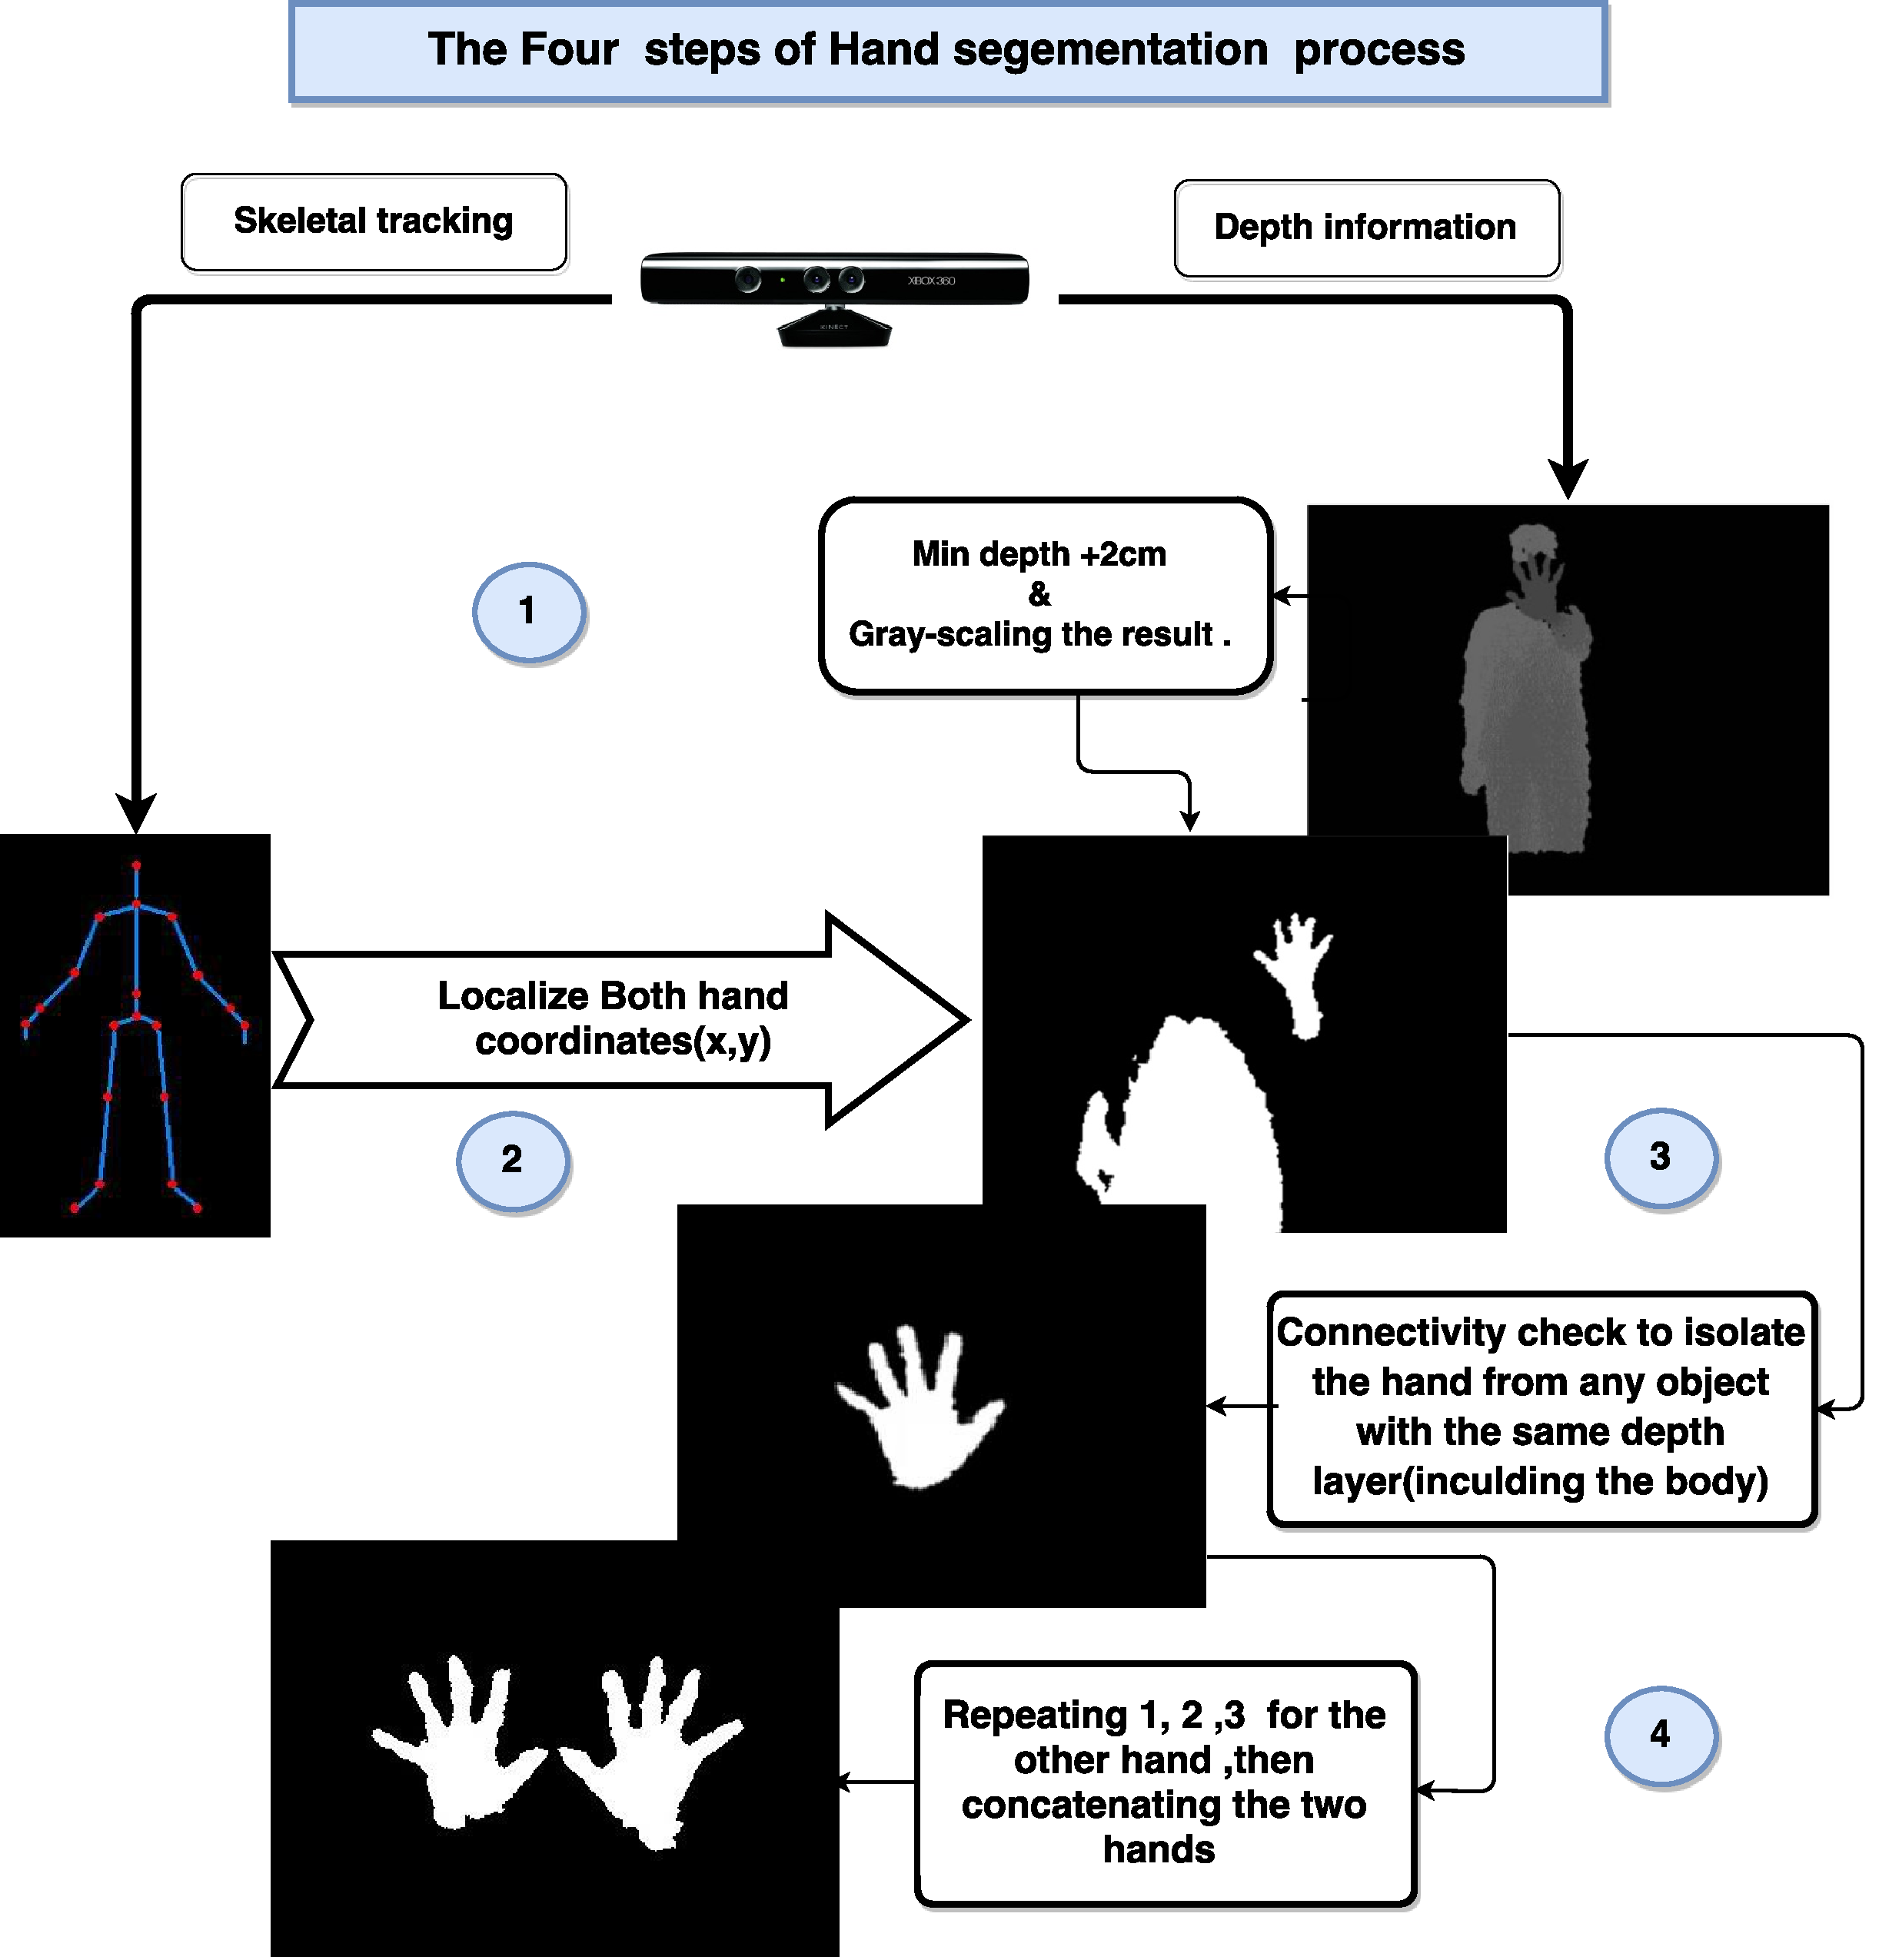
\includegraphics[width=18cm, height=16cm ]{img/preprocessing.pdf}
\caption{result after applying connectivity for both hands  }
\label{fig:preprocessing}
\end{figure}

\textbf{ motion capturing of hand articulation is a challenging task, since the hand presents a motion of high degrees of freedom (rotation variance). Additionally, Our system is based on relative depth which allow user to move around the camera This throws a problem of scale variance}, To solve these issues We chose the best feature descriptor that are most suitable for such a task,which are  SIFT AND SURF descriptor that are both Scale invariant and rotation invariant.

in the next section we will build the recognition System using these descriptors.

\section{ Gesture recognition using surf and sift}


\subsection{Feature Descriptor selection :}
in order to Choose the most suitable descriptor for our HGR system we must choose wisely what kind of descriptor can give us the most promising results, as such  HOG(histograms of oriented gradients) feature that  has been introduced into \textbf{gesture recognition }, but the HOG features is not ideal for gesture recognition for it's computation in dense grids at some single scale without orientation alignment. SIFT ( Scale Invariant Feature Transform) has shown good achievement over the years in object recognition and thus is a good candidate for our system.\\ The contribution of this project is that we propose surf and sift feature descriptors of hand gesture images and then bag of visual words are to map these descriptors to a dimension vector and a  support vector machine(SVM) classifier is then  trained to recognize hand gestures.
\begin{enumerate}
\item We show that this model is not only effective for common hand gestures dataset, but also achieves good  recognition rate for depth data collected by Kinect sensor.
\item Hand gestures training images can be represented by sets of keypoint descriptors generated by SIFT or SURF, but the numbers of keypoints from the images are \textbf{different and lack meaningful ordering }. This creates difficulties for machine learning methods. To address  this problem, we use the bag-of-words ( also called bag of features ) approach.

\end{enumerate}

\subsection{Bag Of visual Words Model}

\begin{wrapfigure}{r}{0.28\textwidth}
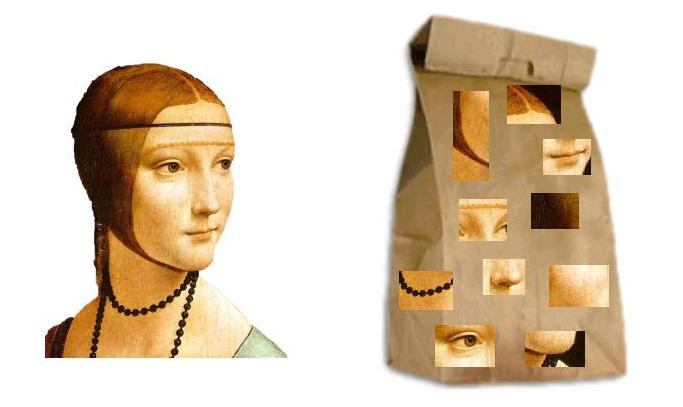
\includegraphics[width=0.25\textwidth]{img/codebook.jpg}
\caption{Example of Visual words in a codebook}
\label{fig:coodbook}
\end{wrapfigure}

\textbf{Bag-of-words} (also called bag of features) is one of the most famous approaches in computer vision, the idea is almost like a  dictionary of local interest points (keypoint ) of an image or images’ datasets. where the object is  represented as a bag of visual words fig [\ref{fig:coodbook}].
Basically, the important points in images are the visual words. These points are features  and they are discriminative and very stable to rotations changes and scale changes. 
The BoW model can be used for image classification, by building a vocabulary database(codebook) of many visual words and represent every image as a histogram of the frequency words that  are in  the image. In order to use BoW for image classification, these features need to be extracted and then we need to generate a codebook, and a histogram afterwards. To retrieve these features,we use some of the local features descriptors such as (SIFT, SURF,HOG,GLOH,ORB,FAST..).
Following this step, each image is a collection of  vectors of the same dimension, \textbf{in which the order of different vectors is not important, but the sets diversify in cardinality and lack significant ordering}. This creates difficulties for learning methods (e.g., classifiers) that  require feature vectors of  \textbf{fixed dimension}  as input.
the vector quantization technique regroups ( clusters)  the keypoint descriptors in their feature space into large sets using the clustering algorithm K-means and encodes each keypoint to the index of the cluster to which it belongs. Each cluster is a visual word that represents a specific local pattern shared by the keypoints in that cluster. Thereby the clustering process generates vocabulary of visual words describing local patterns in images. The codebook size is determined by the number of clusters, therefore, each patch in an image is mapped to a particular codeword.


\subsection{keypoint descriptor Clustering }

\begin{enumerate}
\item \textbf{Feature extraction and description.} It is to extract a representative local features from an image as a description (surf or sift ).
\item \textbf{ Dictionary}
using K-means to cluster Surf or Sift features into K centroids this process is detailed in section [\ref{kmeans}],  Once Clustering is done, each feature vector (keypoint) is assigned to one and only one cluster center that is in the nearest distance with respect to the Euclidean metric in 64 / 128 dimensional feature vectors. The keypoints that are assigned to the same cluster center will be in the same subgroup so that after clustering we have k disjoint subgroups of keypoints. Therefore k-means clustering decreases dimensionality for every training image with n keypoints (n $\times$ m)) to 1 $\times$ k, where m is number of feature descriptor can be either 63 or 128, k is number of clusters.
\item \textbf{ Generating bag-of-features} in this process we generate a bag of features for input images, That means, each keypoint, extracted from input  image, will be represented by one component in the generated bag-of-feature vector with value equal to the index of the
centroid in the cluster model with nearest Euclidean distance. Figure \ref{fig:histo} shows the process of generating the bag-of-features 

\end{enumerate}


\subsection{classification algorithm }

\textbf{Training Processes are as follows }:


\begin{enumerate}
 \item extracting SURF and SIFT features from training samples with different scales and  orientations.
 \item applying  K-means clustering on the training images will help build the Visual words each visual words is considered as centroid of a subgroup of the same Features, Now we can generate bag of features ( histogram of visual words ) for training images where each keypoint will be extracted from training image, will be represented by one component in the generated bag-of-feature vector with value equal to the index of the centroid in the cluster model with nearest Euclidean
distance this basically means getting frequencies of Visual words in the Current image, to have better visualization  about this step see the Figure \ref{fig:histo}

\begin{figure}[H]
\centering
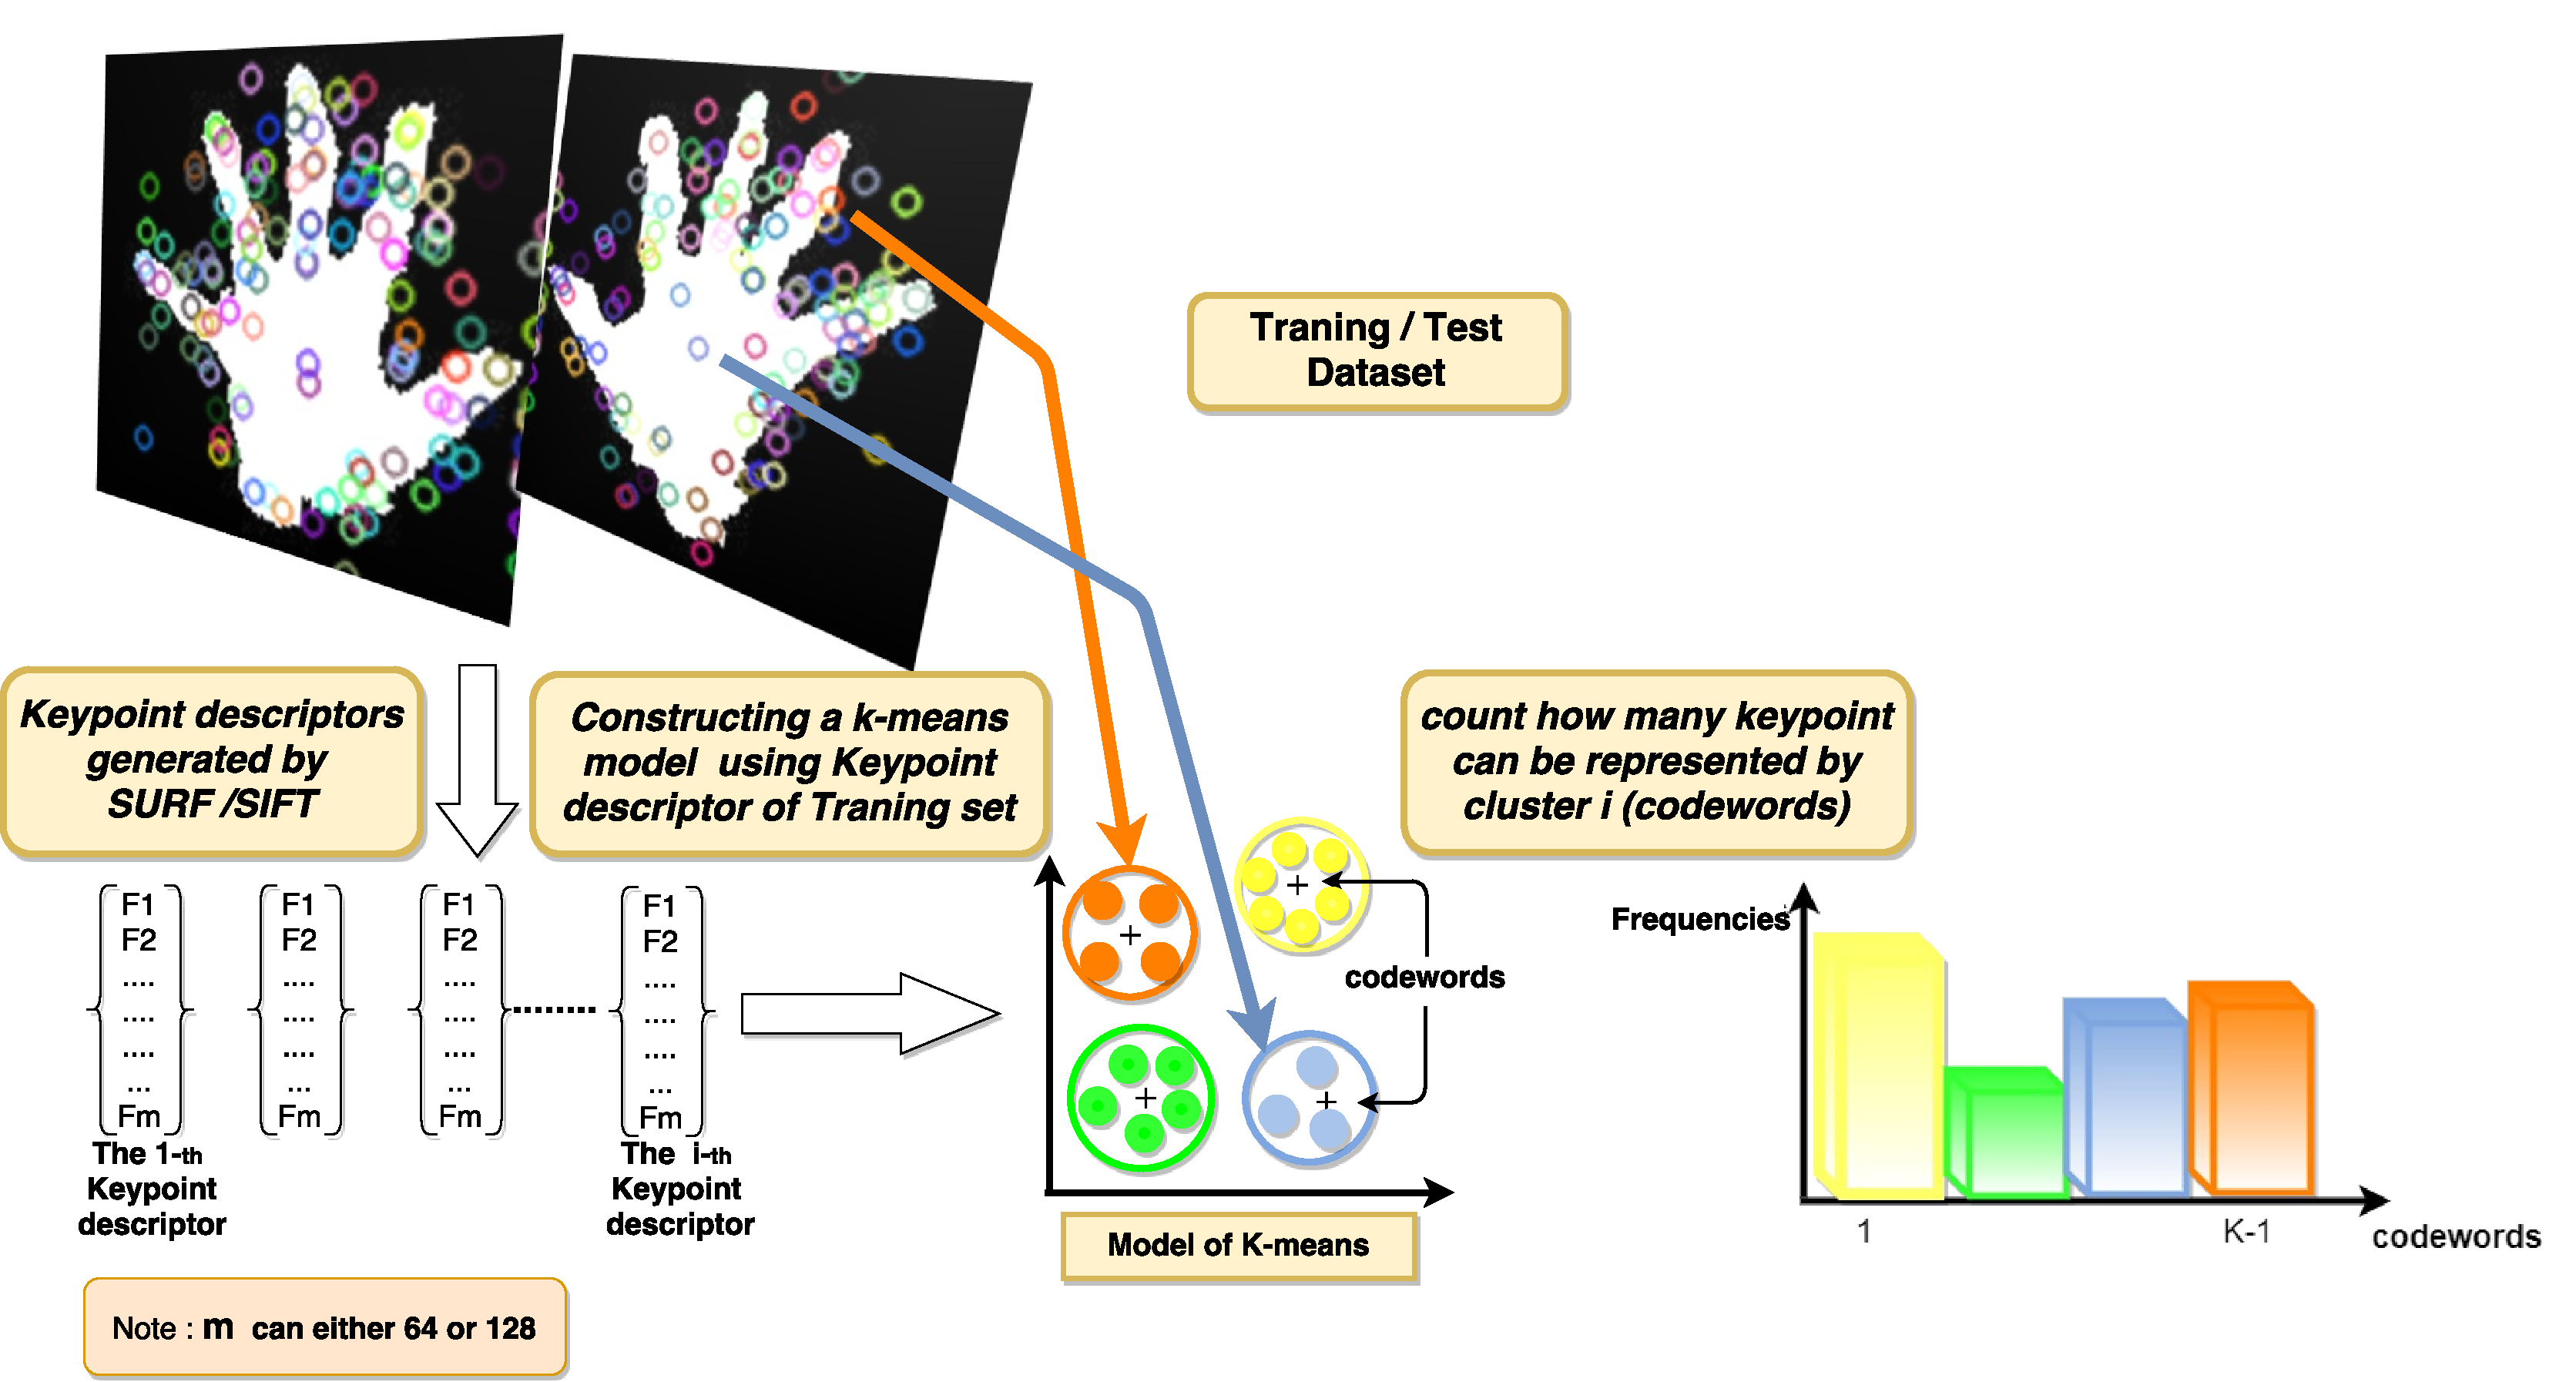
\includegraphics[width=18.5cm, height=11cm ]{img/bow/transparantnewhistogram.pdf}
\caption{ generating histogram for training image and test image by Mapping keypoint into Bag-of-Features space }
\label{fig:histo}
\end{figure}

\item SVM uses a non-linear mapping to transform original training dataset into higher dimension and searches for a linear optimal
separating hyperplane. since our Gesture can have the same shape and certainly often have the same features for two different gestures  this will make Linear separation Hard and can results in false results the kernel method can be used in our case  to transform data  in to higher dimension space in which they are separable. This process will allow classification of multiple classes (16 class ) 
\end{enumerate}


\textbf{validation :}
we used K-fold cross validation method to tune the parameters of our SVM, Using both linear and RBF kernels, Also K that represents Number of clusters plays a role in tuning our model, the result will be shown and discussed in the next section \ref{resultssvm} 



\textbf{Classification process: }
\begin{enumerate}
    \item Extract Keypoint using surf and sift to the test images.
    \item  representing test images by Histogram
    \item using the trained SVM classifier to obtain a classification result.
    
\end{enumerate}

the following Figure \ref{fig:algo1}  summarize the whole  process :

\begin{figure}[H]
\centering
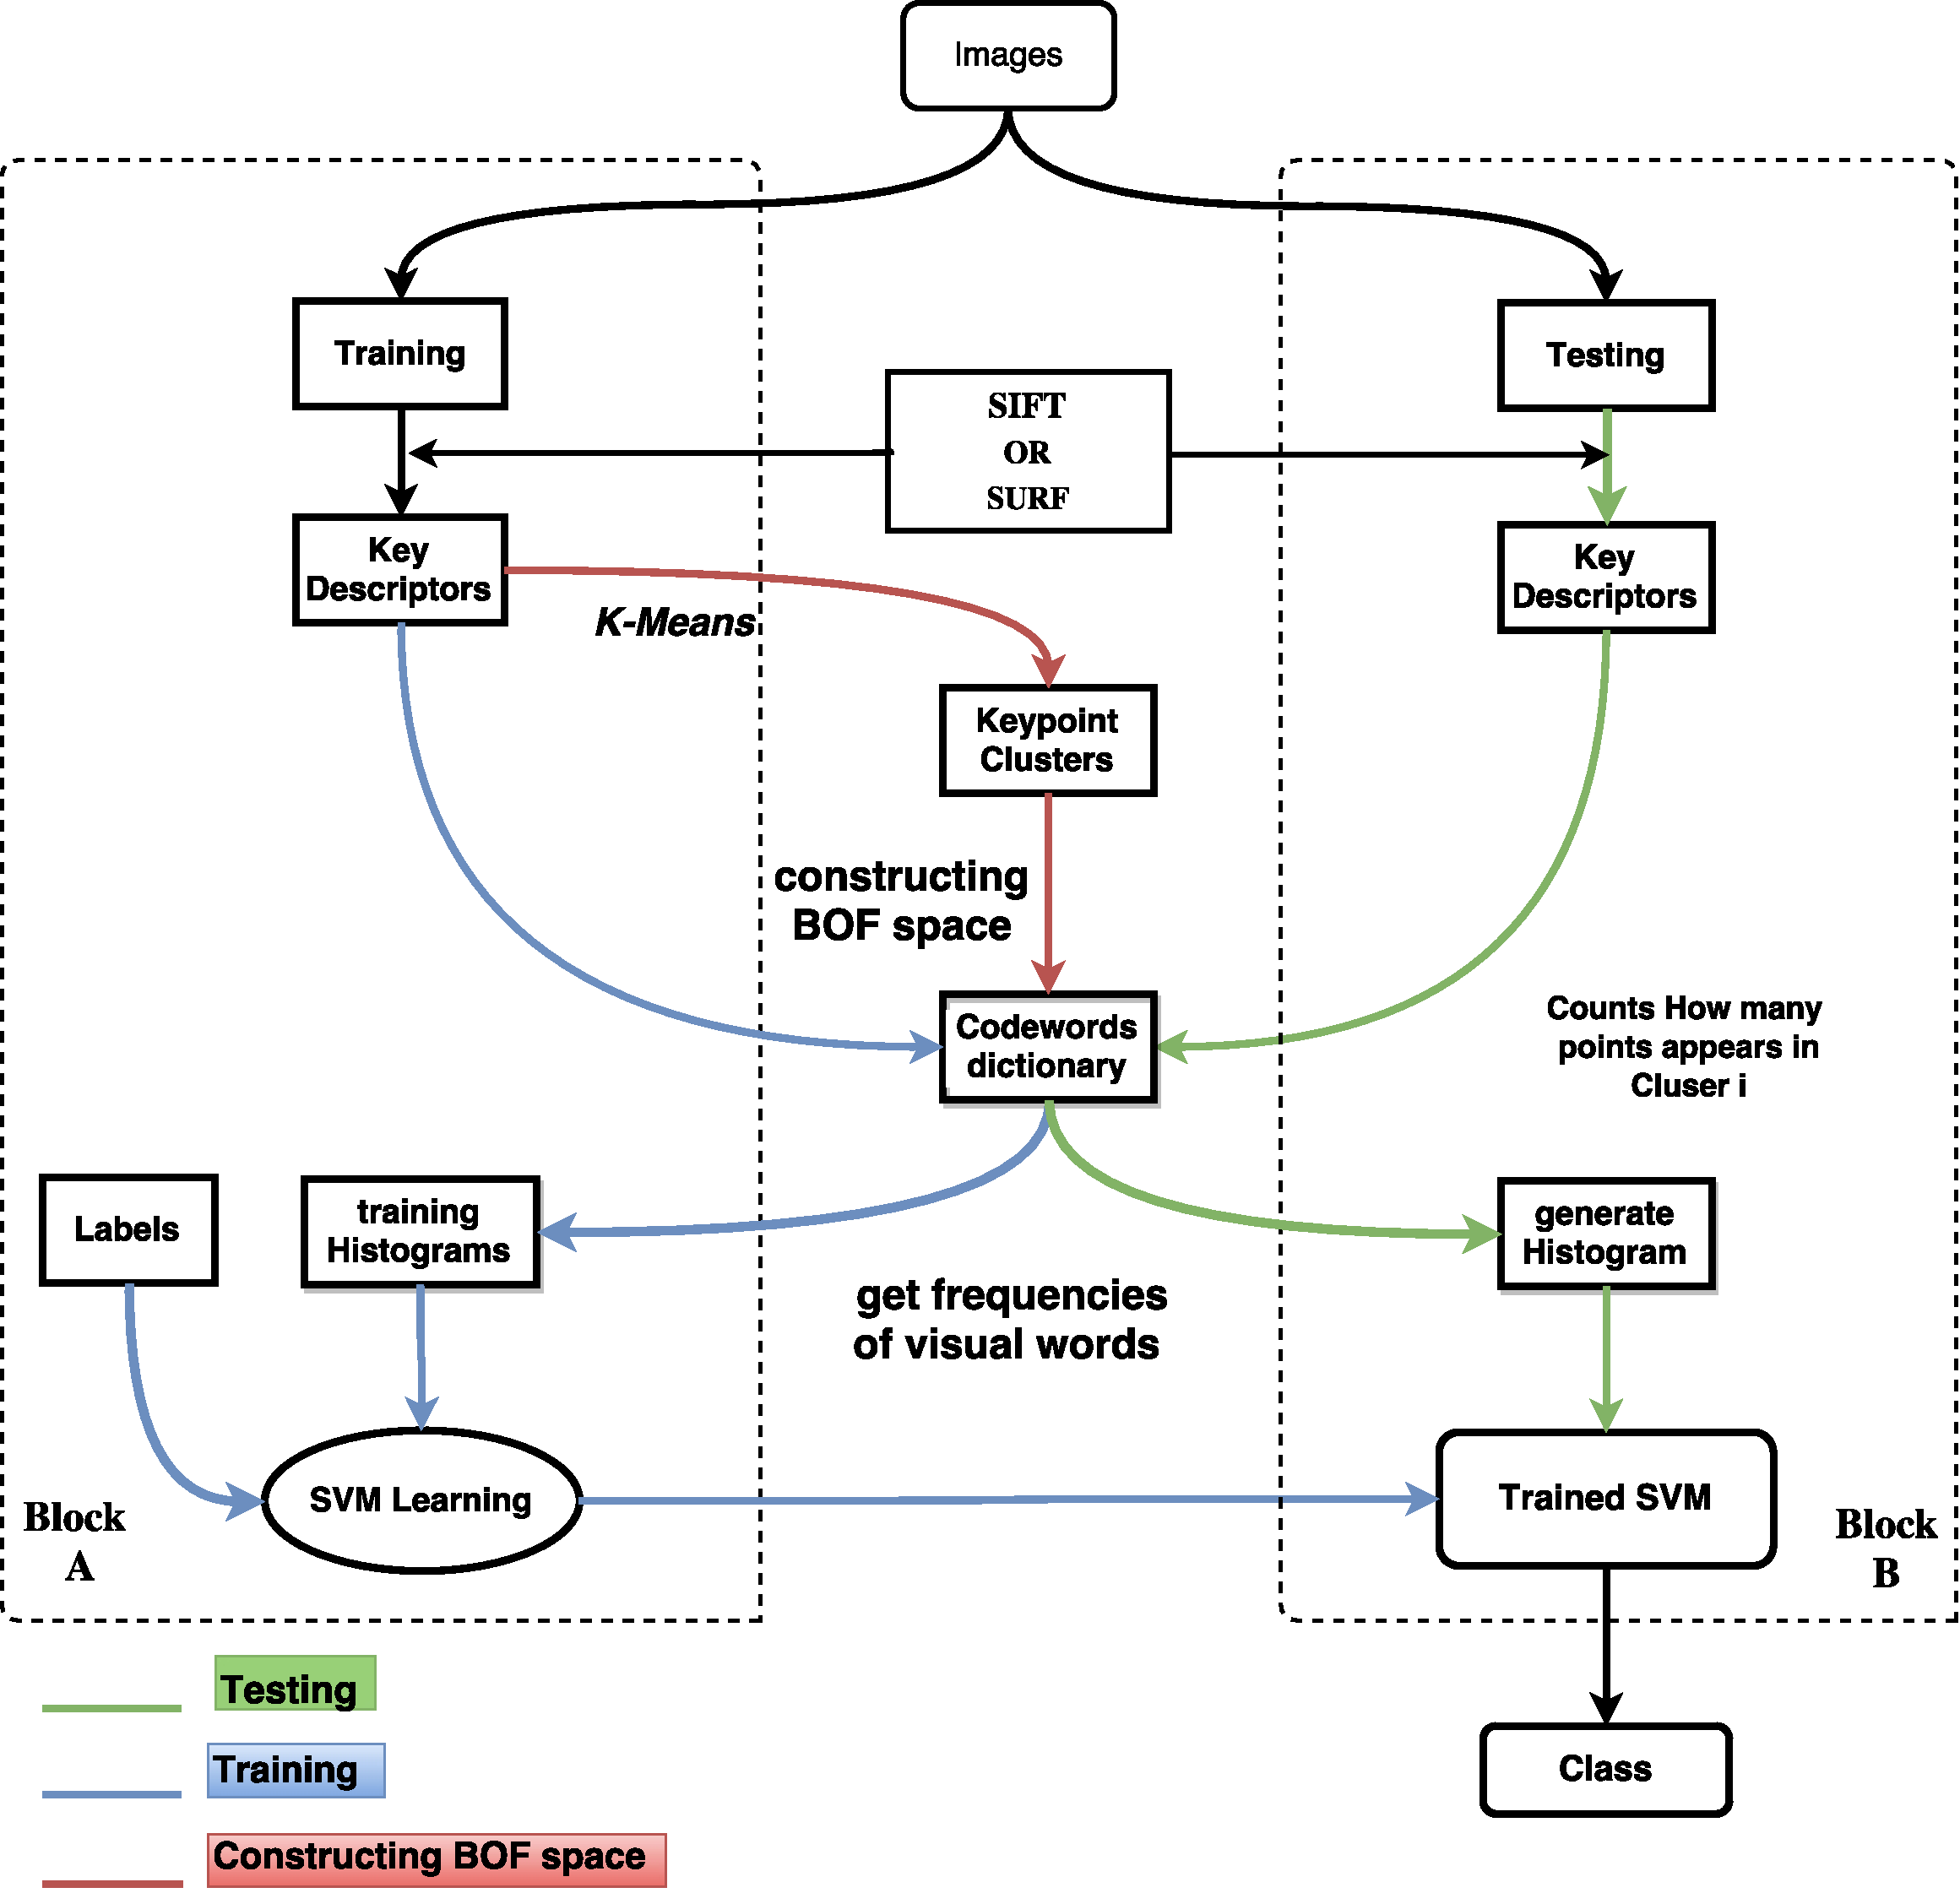
\includegraphics[width=17cm, height=17cm ]{img/bow/mynewalgo.pdf}
\caption{Flowchart for the structure of the algorithm, in block (A) the Extracted Keypoints  are Clustered to i Vocabulary and generate a codewords dictionary,then compute a histogram using visual words ( vocabulary ) for all the training samples these histograms are then fed to an SVM for classification, in Block (B) test images are converted to histogram representation by counting how many keypoints appeared in cluster i,  and then classify the results using the trained SVM }
\label{fig:algo1}
\end{figure}




\subsection{SIFT and SURF  Experimental Results}\label{resultssvm}
in this section we are interested in maximizing the performances of SVM, using K-cross Validation to make model selection, with  K=10 for cross Validation which has ensure us great tuning for our models parameters,
we have chose AUC of ROC curve  to be our main Evaluation Metric since The method can be used for binary classification, therefor we used \textit{one versus all} method to convert the problem to a binary task.

\textbf{Dataset division :}

we took 500 image for each gesture, we divided our dataset into three partitions, training set, validation set,and Test set.

\begin{itemize}
    \item training set :
         300 images for each gestures. with total of 4800 image
    \item validation set :
         100 images for each gestures. with total of 1600 image
    \item test set :
         100 images for each gestures.with total of 1600 image
\end{itemize}



\subsubsection{ SVM performance variation in function of the codebook's size }
The codebook size will be determined depending
on the type  of the data processed. There will be a sort of
compromise  for choosing number of clusters (size of codebook). If it is too large, then there will be quantization artifacts and overfitting because of insufficient samples of the keypoints extracted from the training image. If it is too small, then each bag of words vector will not represent all the keypoints extracted from its related image.

since the structure of our data is unique and has not a lot of keypoint variations, as a matter of fact the hands are the only object detected in all the scenes. so we will start with a  small number for k  and change it until finding a reasonable  AUC ( note : size of codebook is in fact the number of clusters used in K-means).

\begin{figure}[H]
\centering
\includegraphics[width=18cm, height=5cm]{img/bow/dictionnary1.png}
\caption{}
\label{fig:codbooksize}
\end{figure}

\subsubsection{SVM linear kernel}

the feature vector resulted  by surf and sift  in the training set is  519523 for SURF  and 208397 for SIFT, using  bag of feature we reduce it to (4800 $\times$ 500) where 4800 is the number of all training set and 500 is the number of codewords in our codebook  that represent for SVM the number of features, even with dimensionality reduction it is still a big feature vectors to train, thus the choice of linear kernel that generate a limited number of support vectors.


\subsubsection{Surf performance: }
first we varied the Hyper-parameter \texttt{C}, in order to to find an optimal value that maximize SVM performance, the following figure \ref{fig:C} illustrate the variation  of the average AUC of ROC in function of C variations.

\begin{figure}[H]
\centering
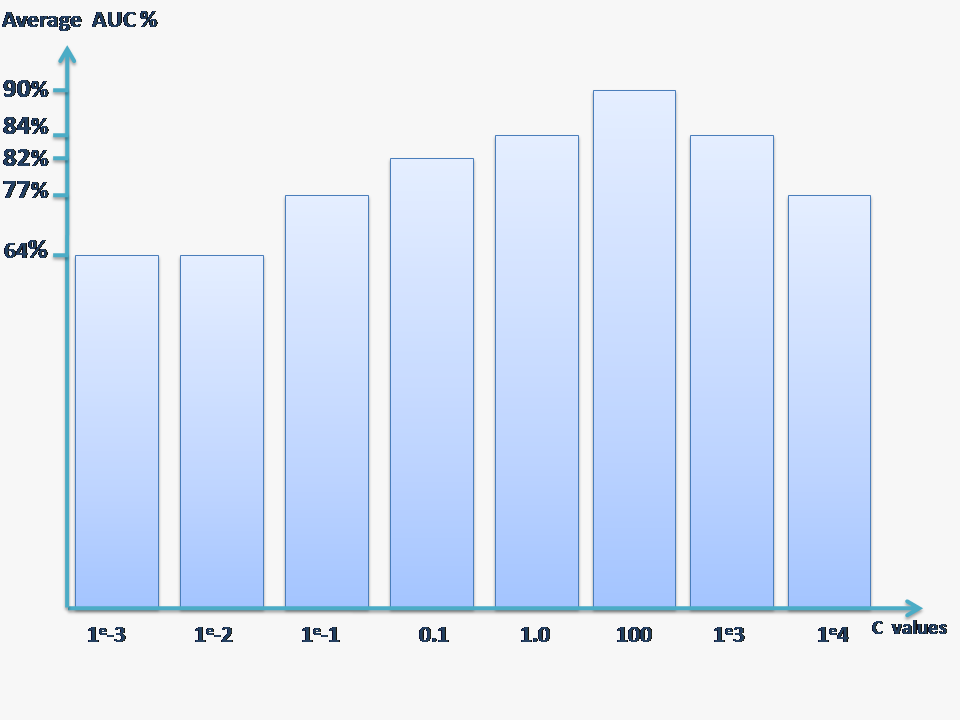
\includegraphics[width=0.56\textwidth]{img/C_values.png}
\caption{the choice of hyper-parameter C }
\label{fig:C}
\end{figure}

C $=$ 100, proved to be the best for linear kernel that scored 90\% Average AUC, thus it was chosen as our Hyperparameter for our model.


the next figure is a representation of ROC curves of Linear Kernel with different C :

\begin{figure}[H]
\centering
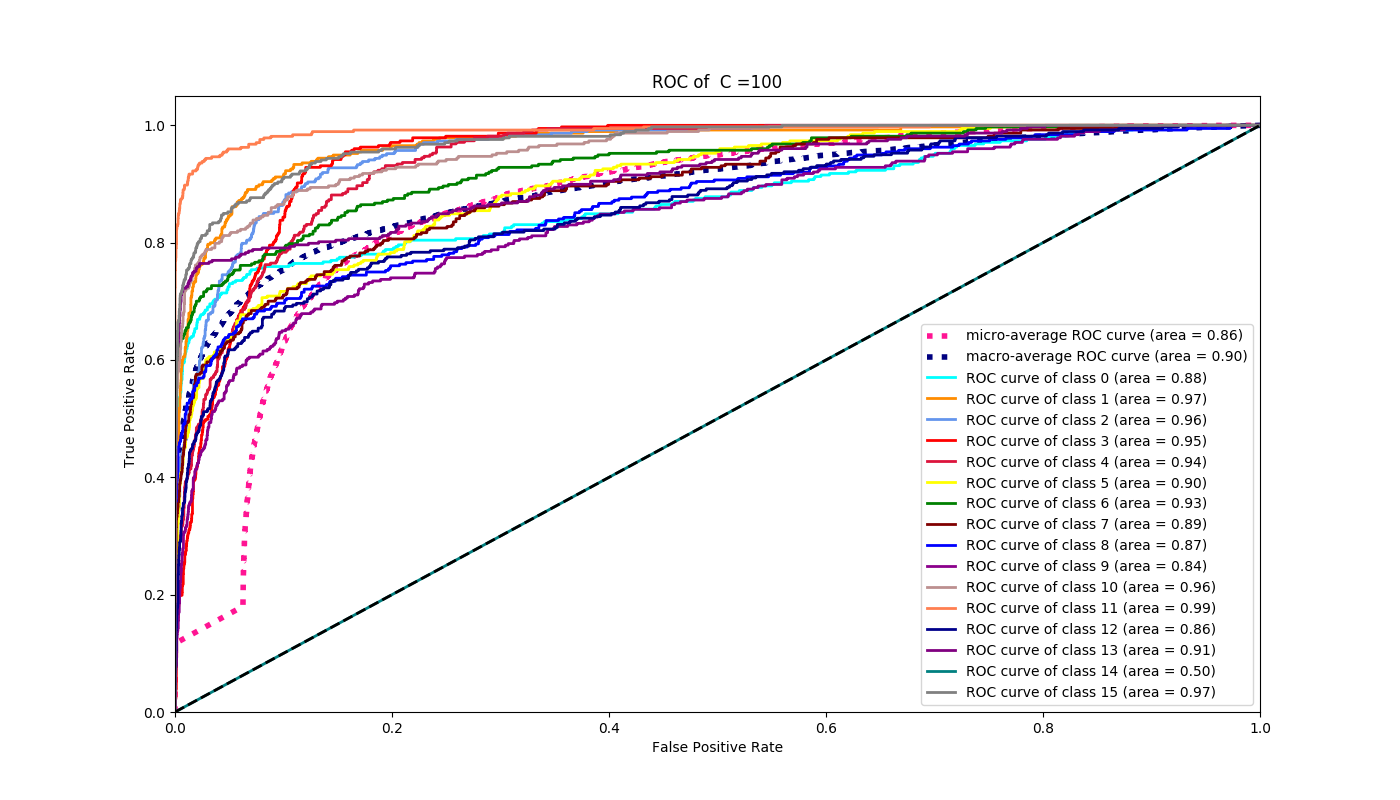
\includegraphics[width=16.5cm, height=11cm]{img/roc/LINEAR_svm_onevsal_ROC_class_C100.png}
\caption{ROC of 16 gestures with  C = 100}
\label{fig:roc}
\end{figure}

\textbf{interpretation }
as shown in the figure above the average AUC is equal to 90 \%
that represent the  overall estimation of our classifier to rank positive data ( in our case is the gesture X $\in$ [0,15]) higher than a negative data ( the rest of gestures excluding the chosen gesture X ),  for instance the gesture 11 that corresponds to gesture V  that has an AUC equal to 99\% this means the classifier can perfectly classify V  among the rest gestures, however the classifier can perform poorly in the case of gesture 14 ("M")with an AUC of  50\%  this means the classifier can  expect  as many gesture M  as other gestures. 

\subsubsection{Sift performance : }
As for sift the optimal value for C is  1.0, to find the best hyperparameter that maximize the linear kernel we varied C and calculates the average ROC AUC fig [\ref{fig:Csift}] :

\begin{figure}[H]
\centering
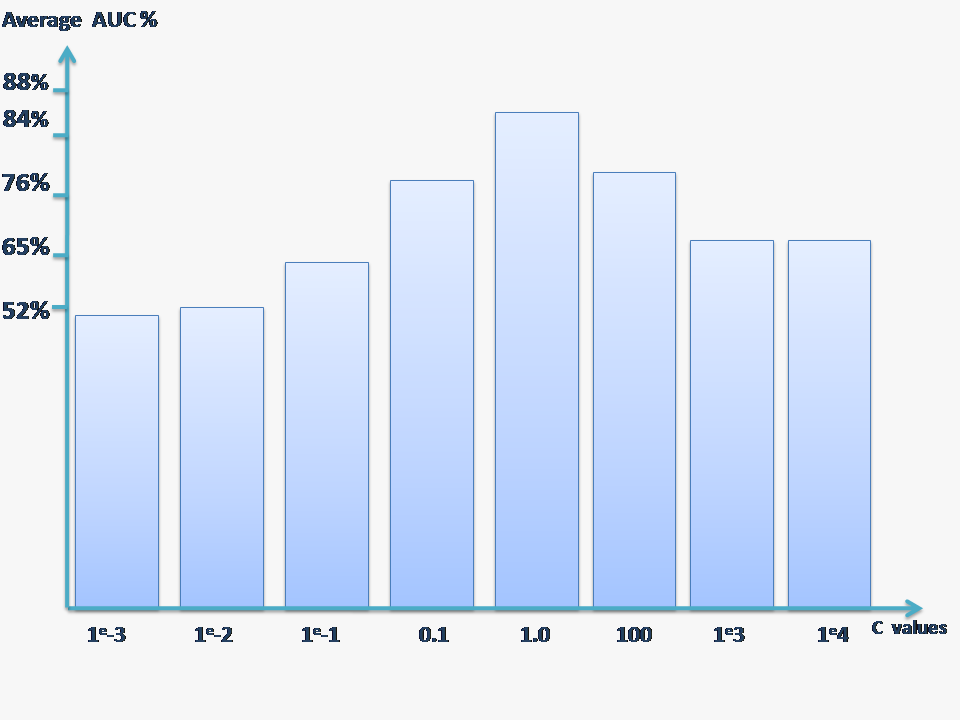
\includegraphics[width=0.6\textwidth]{img/roc/sift_C_values.png}
\caption{the choice of hyper-parameter C }
\label{fig:Csift}
\end{figure}

Next we present ROC curve of 16 gestures with  C= 1.0 using Sift features. 

\begin{figure}[H]
\centering
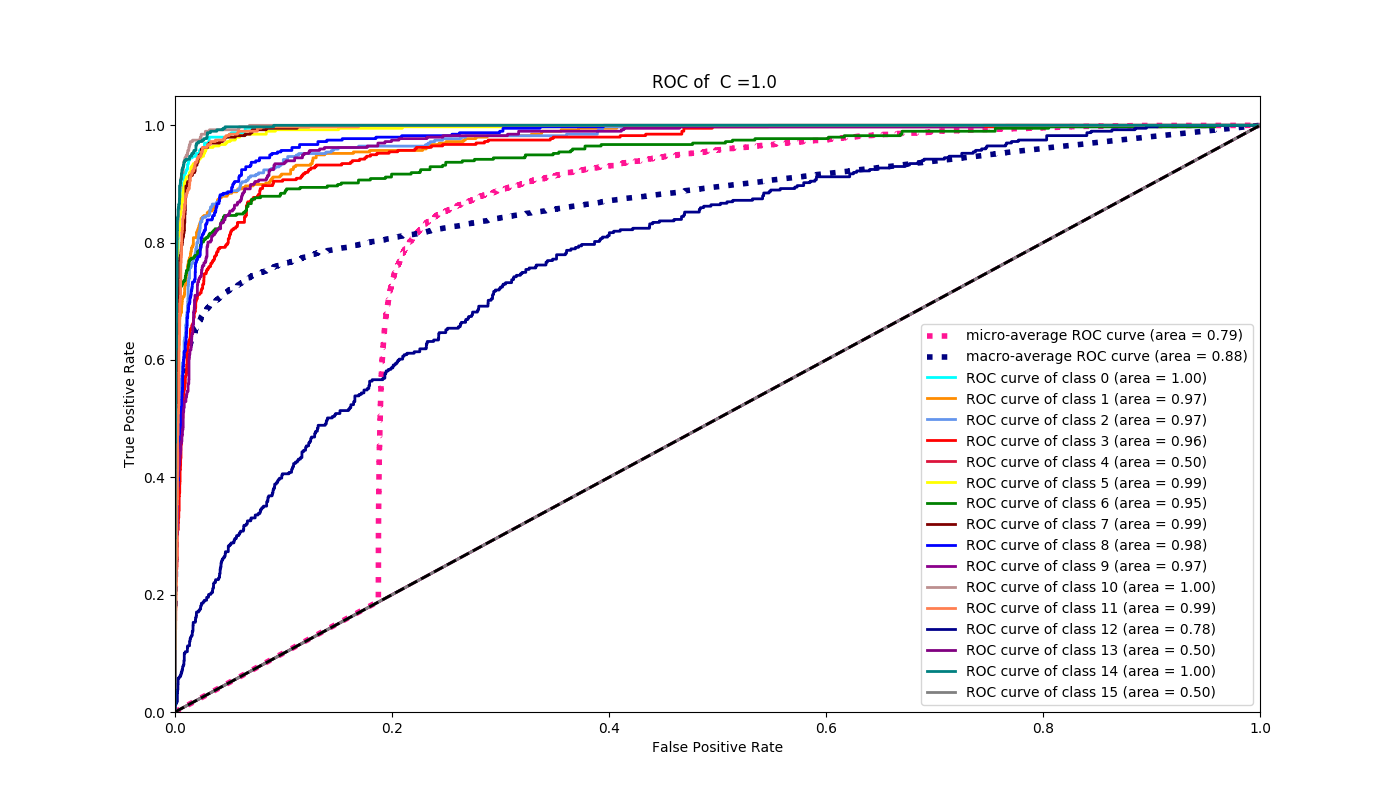
\includegraphics[width=16cm, height=12cm]{img/roc/sift_ROC_class_C.png}
\caption{ROC of 16 gestures with  C = 1.0 }
\label{fig:rocsift}
\end{figure}

\textbf{interpretation :}
The average AUC is 88\%, under this performance the class  13,14,4 that corresponds to gestures ( "M", "O", "E" ), this means the classifier can give random guessing and we expect it to classify "M","O","E" as equally as to all the other gestures. But the classifier was able to achieve good result in almost  all other gestures.


\subsubsection{SVM RBF kernel}

for RBF kernel, we have two parameters to tune our model with, the hyperparameter C and the parameter $\gamma$. we have varied the C in the interval of [$10^{-3}$,0.01,...,$10^{7}$] and $\gamma$ in [$10^{-5},....,10^{3}$], the best parameters were found are C $=$ 1000.0, $\gamma$ $=$ [0.1,1.0,0,10]. these values gave a performance of 98\%.

\subsubsection{Surf performance : }

\begin{figure}[H]
\centering
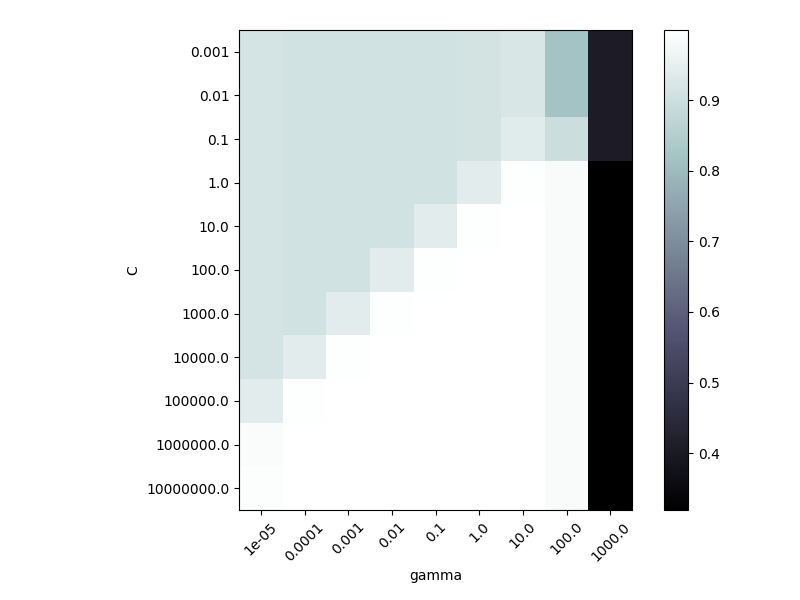
\includegraphics[width=0.71\textwidth]{img/grid/grid_searchbone.png}
\caption{Gridsearch for optimal C and $\gamma$}
\label{fig:grid}
\end{figure}



the following figure is a representation of ROC curve for C $=$ 1000.0, and $\gamma$ $=$ 0.1.

\begin{figure}[H]
\centering
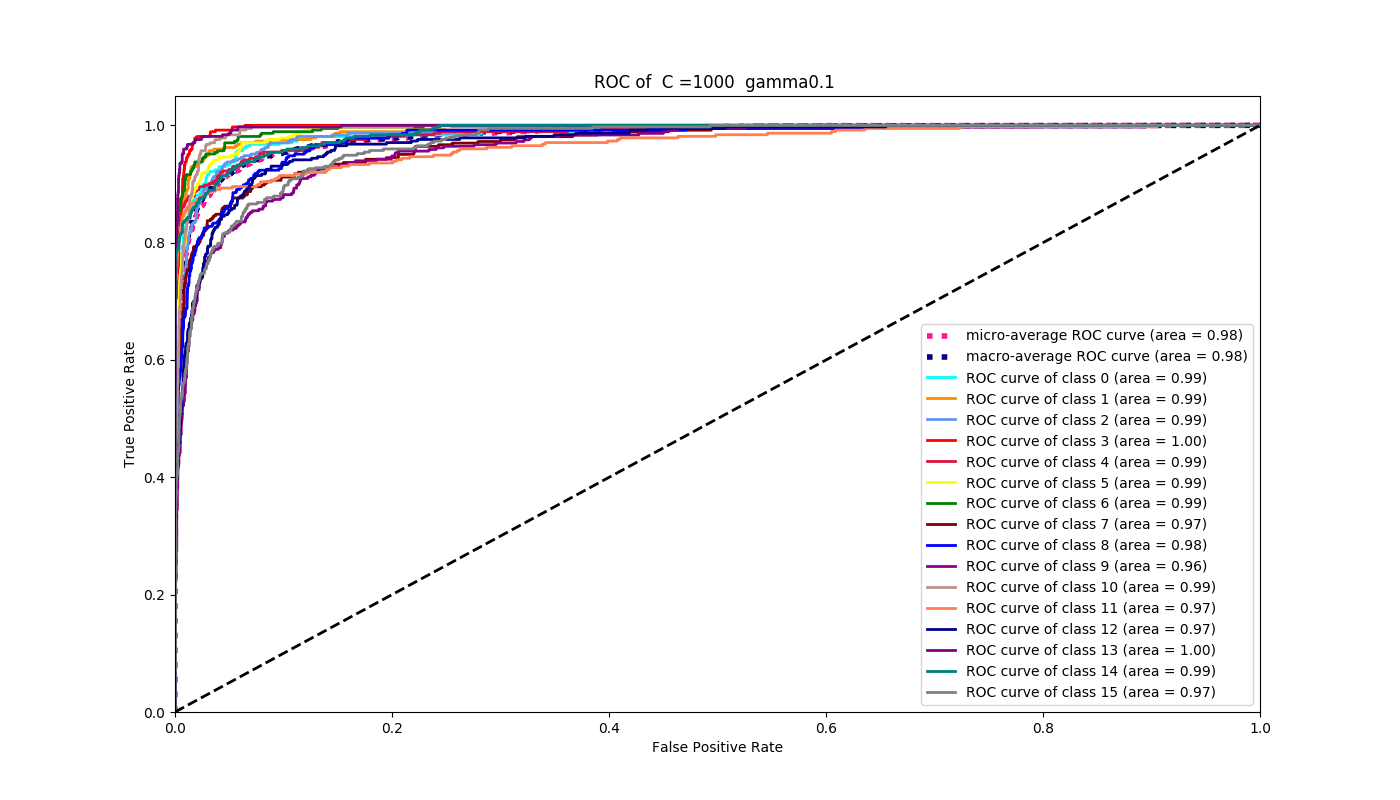
\includegraphics[width=16.5cm, height=10cm]{img/roc/RBF_C1000_gamma01.png}
\caption{Roc for RBF kernel with C= 1000.0 and gamma = 0.1}
\label{fig:rbf0}
\end{figure}
the average AUC is 98\% this describe the probability to classify a gesture X $\in$ \{ gestures\} against other gestures $\in$ \{\{gestures\} - \{X\} \} is almost ideal.
Now let's see the  ROC curve for C= 1000.0 and $\gamma$ = 1.0, that gave an Average AUC of 98 \% as well.
\begin{figure}[H]
\centering
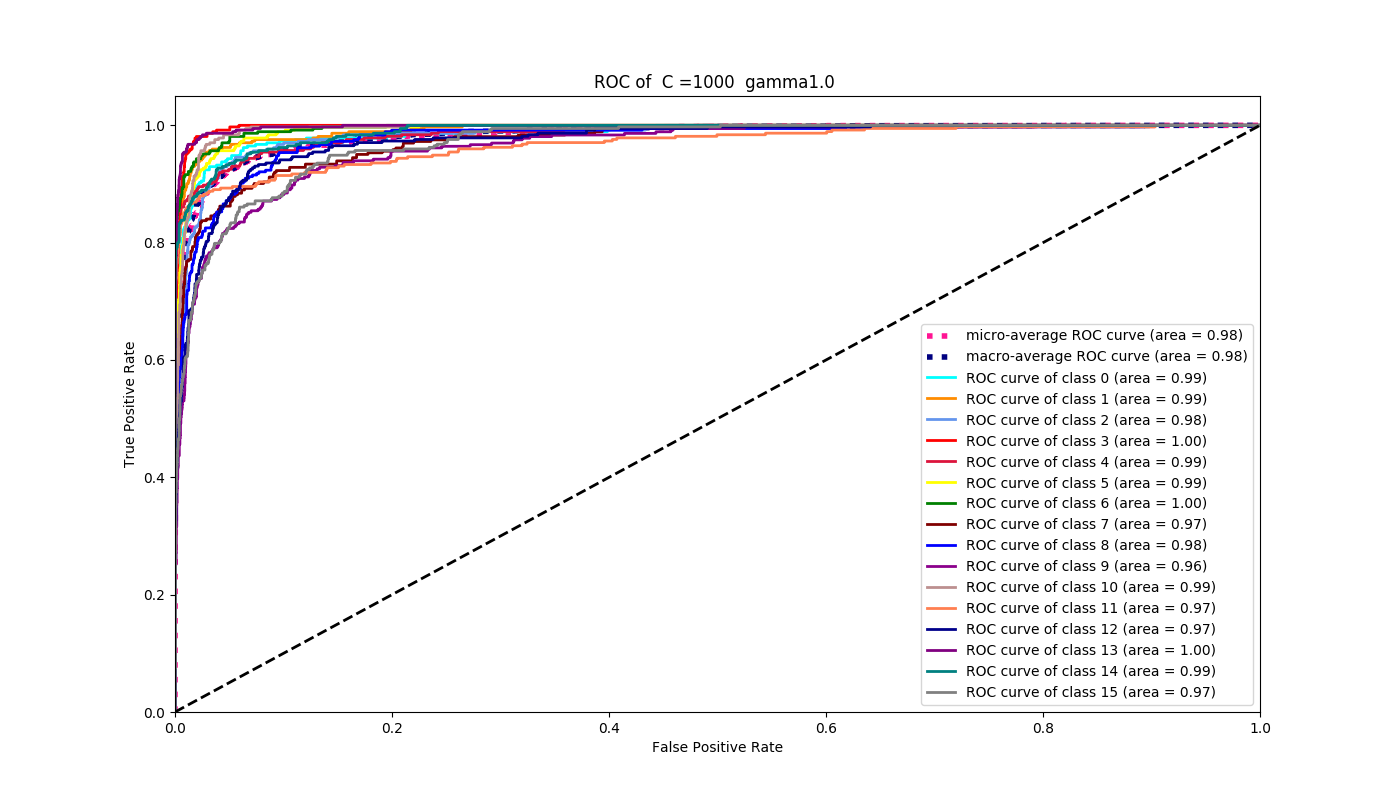
\includegraphics[width=16.5cm, height=11cm]{img/roc/RBF_C1000_gamma10.png}
\caption{Roc for RBF kernel with C= 1000.0 and gamma = 1.0}
\label{fig:rbf1}
\end{figure}

in fact the best optimal gamma was between [0.1,1.0], we have choose C$=$ 1000.0, $\gamma$ = 1.0 for our RBF model.

\subsubsection{Sift perforamnce :}



the following figure is a representation of ROC curve for C $=$ 1000.0, and $\gamma$ $=$ 0.1.

\begin{figure}[H]
\centering
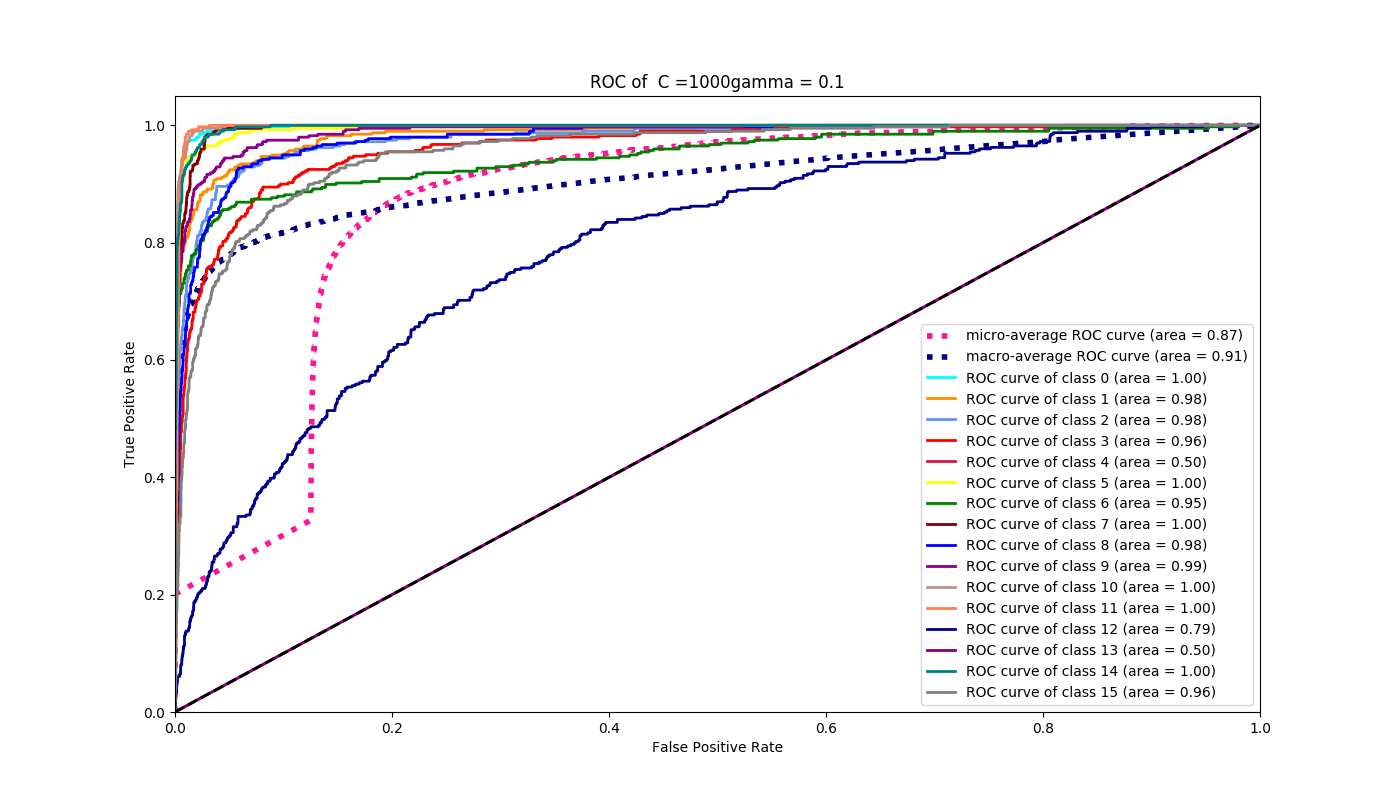
\includegraphics[width=16.5cm, height=11cm]{img/roc/sift_ROC_class_C1000gamma.png}
\caption{Roc for RBF kernel with C= 1000.0 and gamma = 0.1}
\label{fig:rbf2}
\end{figure}


\subsubsection{comparing results  } 

 We found that SURF feature descriptors are more appropriately for visual
hand gesture recognition than SIFT feature descriptors.
SIFT is  slow which  gave lag during feature extraction. on the other hand SURF performs well on Depth and blurry images and is typically 2 to 3 times faster than SIFT as shown in the table below. We took 4800 images of 200 images from each class ( 16 $\times$ 300 ) and registered  the time required for extraction and description  by SURF and SIFT.
\begin{table}[!h]
\centering

\begin{tabular}{c|c|c|ll}
\cline{2-3}
\multicolumn{1}{l|}{\textbf{}}                                                                                                                      & \textbf{SIFT}        & \textbf{SURF}                            &  &  \\ \cline{1-3}
\multicolumn{1}{|c|}{\textbf{\begin{tabular}[c]{@{}c@{}}Average time (in seconds ) consumed for \\ features detection and description Per Image \end{tabular}}} & \textbf{0.30s} & \multicolumn{1}{l|}{\textbf{0.12s}} &  &  \\ \cline{1-3}
\multicolumn{1}{|c|}{\textbf{number of features extracted per image }}                                                                                         & \textbf{43}        & \textbf{107}                            &  &  \\ \cline{1-3}

\end{tabular}
\caption{Average speed time consumed for features detection and extraction And accuracy for SURF and SIFT applied on a set of 4800 images for 16 different gestures }
\label{siftvssurfacc}
\end{table}

Surf Can be 3  times faster than sift also Surf Was capable of describing Gesture keypoint better than sift by difference of 50 keypoints  it can gives an Idea about the descriptor that suits best our data and can extract as much information as needed for recognition. The average ROC AUC  in sift is 88\% in linear kernel while surf scored 90\%, and as for RBF kernel still surf was the winner by 98\%  against 91\%.
For all the Reasons cited above  we found SURF descriptors to be apt for our application to meet the requirement  \textbf{of a  Real time application} since Sift descriptor can not be used in real time applications however Not with normal machines.

%%%%%%%%%%%%%%%%%%%%%%%%%%%%%%%%%%%%%%%%%%%%%%%%%%%%%%%%%%%%%%%%%%%%%%%%%%%%%%%%%%

\section{gesture recognition using Fourier Descriptor and NN  classifier }

 The use of depth image has benefit
in segmenting hand image rather than color-based
segmentation, segmentation in depth image is more robust
since the lighting variation does not affect the image quality.
 Fourier descriptors represent feature of each hand gesture as Unique signature As long as the shape (images ) are different from each others.
Generally, this section is separated into two phases:
dictionary build phase and classification phase. \\In the
dictionary build phase, the Fourier descriptors of each
character are stored into a database to develop gesture
dictionary. The gesture dictionary and comparison methods are
derived from \cite{clif}.\\ The classification phase has the similar
step, except that the Fourier descriptors are compared with the
dictionary using distance metric as classification methods.
The result of classification phase is the meaning of the
acquired gesture sign.
\texttt{For more details about the algorithm used for this project please check the section \ref{FDT}
}

\subsection{Classification }
Now we have a set of features for each image and the next
step is to train a classifier to classify the different hand shapes
used in testing. the classifier used in for Fourier descriptor is based on Euclidean distance which is a very simple way for
classification.\\
Classification using Euclidean Distance: The set of
features induces a distance on the shape space, which is given
by the Euclidean distance: 
$$d(f_{1},f_{2}) = \sqrt{\sum_{k=0}^{N-1} |f_{1}(k)-f_{2}(k)|^{2}}$$\\
\texttt{ Where $f_{1},f_{2}$ are the feature vectors for the two images being
compared. The two vectors with the least distance will have
the same class}\\

The following Figure \ref{fig:dft} summarize the whole process :  
        
\begin{figure}[H]
\centering
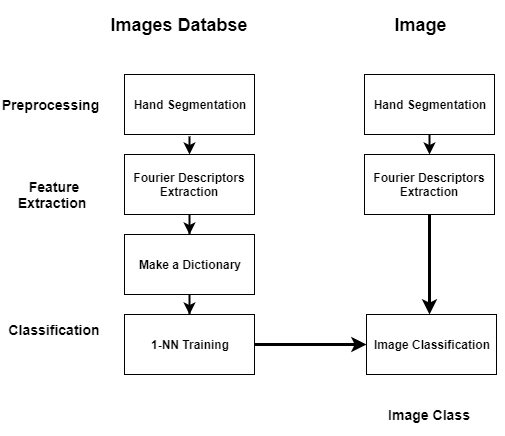
\includegraphics[width=0.8\textwidth]{img/latex.png}
\caption{the architecture used for FDs}
\label{fig:dft}
\end{figure}




\subsection{Fourier descriptor Experimental Results :}

For each shape we select a set of points with the equal point
sampling method. To use DFT we choose a number that is a
power-of-two. We tested the classifiers with initial 128, 64, 32, 16
and 8 points. Those features are used as a training set to be
used in classification. To classify the test image we used the Classifier Nearest Neighbor that uses simple  Euclidean distance, where we calculated the distance between the features of each image in
the test set with the features of the Dictionary.


\subsubsection{Accuracy variation in function of number of Fourier descriptor features : }


// still in the process..


\section{comparing results for FD}




...



\section{Conclusion}


........